\documentclass[../notes.tex]{subfiles}

\pagestyle{main}
\renewcommand{\chaptermark}[1]{\markboth{\chaptername\ \thechapter\ (#1)}{}}
\setcounter{chapter}{5}

\begin{document}




\chapter{Modules Intro}
\section{Module Tools}
\begin{itemize}
    \item \marginnote{2/6:}A fifth week summary has been posted.
    \begin{itemize}
        \item Week 5 content is not in the midterm syllabus.
        \begin{itemize}
            \item In particular, Gauss's Lemma is not on the midterm.
        \end{itemize}
        \item Lecture 5.3 won't even be on the final syllabus.
        \item The techniques are applicable to a variety of problems, though, so it is good to know them.
    \end{itemize}
    \item Today: Modules.
    \begin{itemize}
        \item We depart from commutative rings and return to simple rings with identity to start.
    \end{itemize}
    \item Notation: What kinds of sets different letters denote.
    \begin{itemize}
        \item $A,B$: Rings.
        \item $R$: Commutative ring.
        \item $F,K$: Fields.
        \item $D$: Division ring.
    \end{itemize}
    \item Linear algebra is the study of division rings but only over fields.
    \item Definition of a \textbf{division ring}.
    \begin{itemize}
        \item The only ideals of a division ring are $0,D$, just like with fields.
        \item Linear independence, spanning, basis, etc. all hold in a general division ring; you only need fields for things like JCF.
    \end{itemize}
    \item \textbf{Left $\bm{A}$-module}: An abelian group $(M,+)$ equipped with an action $\cdot:A\times M\to M$ defined by $(a,m)\mapsto am$ (or $a\cdot m$ in the case of potential ambiguity) satisfying the following. \emph{Also known as} \textbf{left module} (over $A$). \emph{Constraints}\par
    For all $a,b\in A$ and $v,v_1,v_2\in M$\dots
    \begin{enumerate}[label={(\arabic*)}]
        \item $a(v_1+v_2)=av_1+av_2$;
        \item $(a+b)v=av+bv$;
        \item $a(bv)=(ab)v$;
        \item $1_Av=v$.
    \end{enumerate}
    \item We need the last one so that multiplication is nontrivial.
    \item A \textbf{right $\bm{A}$-module} puts the scalar on the right. Will we ever consider these??
    \item Notation: For all $a\in A$, define the function $\rho(a):M\to M$ by $\rho(a)v=av$ for all $v\in M$. \emph{Constraints}
    \begin{enumerate}[label={(\arabic*)}]
        \item $\rho(a)$ is a group homomorphism from $M\to M$.
        \item $\rho(a+b)=\rho(a)+\rho(b)$.
        \item $\rho(a)\rho(b)=\rho(ab)$.
        \item $\rho(1_A)=1_{\End(M)}$
    \end{enumerate}
    \item Conditions 2-4 imply that $\rho:A\to\End(M)$ is a ring homomorphism.
    \begin{itemize}
        \item Recall HW1 Q1.14, which led up to the result that
        \begin{equation*}
            \End(M) = \{f:M\to M\mid f\text{ is a group homomorphism}\}
        \end{equation*}
        is a ring with identity under componentwise addition and composition (i.e., $g\cdot f=g\circ f$).
        \item $\End(M)$ is formally defined in \textcite{bib:DummitFoote} at this point!
    \end{itemize}
    \item Going forward, in-class definitions will always match those in the book.
    \begin{itemize}
        \item It's been this way for a while??
    \end{itemize}
    \item Examples.
    \begin{enumerate}
        \item Let $M=A$. Then $\rho(a)b=ab$ for all $a\in A$, $b\in M=A$.
        \item If $M_i$ is a (left) $A$-module for all $i\in I$ an indexing set, then the product $\prod_{i\in I}M_i$ is also an $A$-module.
        \begin{itemize}
            \item The binary operation obeys the product topology: If we denote an element of $\prod_{i\in I}M_i$ by $\prod_{i\in I}m_i$, then we define $\cdot$ by
            \begin{equation*}
                a\cdot\left( \prod_{i\in I}m_i \right) = \prod_{i\in I}(am_i)
            \end{equation*}
        \end{itemize}
        \item Special case of 2: The collection
        \begin{equation*}
            \oplus_{i\in I}M_i = \left\{ \prod_{i\in I}m_i\mid\{i\in I:m_i\neq 0\}\text{ is a finite set} \right\}
        \end{equation*}
        is an $A$-module.
        \begin{itemize}
            \item This is a submodule of Example 2 under the same binary operation.
        \end{itemize}
        \item Special case of 2: $A^m$ is an $A$-module with $a(b_1,\dots,b_n)=(ab_1,\dots,ab_n)$.
        \begin{itemize}
            \item These are considered in much greater depth in \textcite{bib:DummitFoote}.
        \end{itemize}
    \end{enumerate}
    \item \textbf{$\bm{A}$-submodule}: A subgroup $(N,+)$ of $(M,+)$ such that for all $a\in A$ and $\omega\in N$, $a\omega\in N$.
    \item Observation: If $N_1,N_2$ are submodules of $M$, then $N_1+N_2$ and $N_1\cap N_2$ are submodules.
    \item Question (base case): What are the submodules of $A$, itself?
    \begin{itemize}
        \item Left ideals.
    \end{itemize}
    \item \textbf{Module homomorphism}: A function $T:M\to N$ such that $T$ is a homomorphism of abelian groups and commutes with scalar multiplication (i.e., $T(av)=aT(v)$ for all $a\in A$, $v\in M$). In full, we have
    \begin{equation*}
        T(a_1v_1+a_2v_2) = a_1T(v_1)+a_2T(v_2)
    \end{equation*}
    for all $a_1,a_2\in A$ and $v_1,v_2\in M$.
    \item Question: What are all of the module homomorphisms $T:A\to M$?
    \begin{itemize}
        \item If $T(1)=v$, then $T(a\cdot 1)=aT(1)=av$ for all $a\in A$. Thus, we see that defining $T(1)$ is sufficient to define $T$.
        \item In other words, there exists a unique $T:A\to M$ for all $v\in M$ such that $T(1)=v$
        \item This is very related to linear algebra!
    \end{itemize}
    \item Question: What are all linear transformations $T:A^n\to M$?
    \begin{itemize}
        \item Suppose $e_1=(1,0,\dots,0)$, $e_2=(0,1,0,\dots,0)$, etc. Then
        \begin{equation*}
            (a_1,\dots,a_n) = \sum_{i=1}^na_ie_i
        \end{equation*}
        \item Therefore,
        \begin{equation*}
            T(a_1,\dots,a_n) = \sum_{i=1}^na_iTe_i
        \end{equation*}
        \item Take any ordered $n$-tuple of elements in $M$; then given $v_1,\dots,v_n\in M$, there is a unique $A$-module homomorphism $T:A^n\to M$ such that $T(e_i)=v_i$ ($i=1,\dots,n$).
    \end{itemize}
    \item \textbf{Isomorphism} (of $A$-modules): A bijective module homomorphism $T:M\to N$, where $M,N$ are $A$-modules.
    \begin{itemize}
        \item It follows that $T^{-1}:N\to M$ is also a homomorphism.
        \item Note that it suffices to use the bijectivity definition here, not the left and right inverse one.
    \end{itemize}
    \item Proposition: Let $N$ be a submodule of $M$. Then the quotient group $M/N$ has a unique structure of an $A$-module such that $\pi:M\to M/N$ (defined with groups) is an $A$-module homomorphism.
    \begin{proof}
        {\color{white}hi}\par
        \underline{Existence}: For all $a\in A$, we have that $\rho(a):M\to M$ take $\rho(a)N\subset N$. It induces $\overline{\rho(a)}:M/N\to M/N$. Take $\overline{\rho(a)}$, which is scalar multiplication by $a$ on $M/N$.\par
        See Proposition \ref{prp:10.3}.
    \end{proof}
    \item FIT: Let $\phi:M\to N$ be a module homomorphism. Then $\ker(\phi)$ is a submodule of $M$ and $\im(\phi)$ is a submodule of $N$.
    \begin{figure}[H]
        \centering
        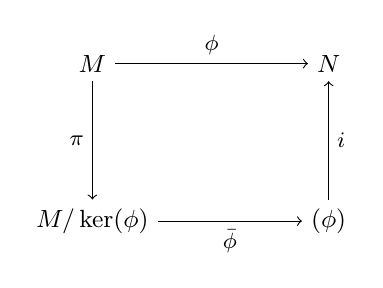
\begin{tikzpicture}[xscale=3,yscale=2]
            \small
            \node (M)  at (0,1) {$M$};
            \node (Mk) at (0,0) {$M/\ker(\phi)$};
            \node (Mi) at (1,0) {$\im(\phi)$};
            \node (N)  at (1,1) {$N$};

            \footnotesize
            \draw [->] (M)  -- node[left] {$\pi$}        (Mk);
            \draw [->] (Mk) -- node[below]{$\bar{\phi}$} (Mi);
            \draw [->] (Mi) -- node[right]{$i$}          (N);
            \draw [->] (M)  -- node[above]{$\phi$}       (N);
        \end{tikzpicture}
        \caption{First isomorphism theorem of modules.}
        \label{fig:FITModule}
    \end{figure}
    \begin{proof}
        See Theorem \ref{trm:10.4a}.
    \end{proof}
    \item Example: $A=\Z$ and $M=\Z/(27)$.
    \item For all of this module stuff, think in terms of fields! If Nori had been couching all of this in terms of vector spaces, we would all get all of this immediately.
    \item Let $n=1$, $(2)\subsetneq\Z$. Then $m=n$ does not imply $M=R^n$.
    \item Submodules of $R$ are ideals. Thus, in a PID, they're principal ideals.
    \item Theorem: Let $R$ be a PID. Then every $R$-submodule of $R^n$ is isomorphic to $R^m$ for some $0\leq m\leq n$.
    \begin{proof}
        We induct on $n$. For the base case $n=1$, let $M$ be an $R$-submodule of $R^1$. As a submodule of a ring, $M$ is an ideal. Thus, since $R$ is a PID, we know that $M=(b)$ for some $b\in R$. If $b=0$, then we're done (pick $m=0$). Thus, assume $b\neq 0$. Consider $T:R\to(b)$ given by $T(a)=ab$ for all $a\in A$. We have that $T$ is onto. From the fact that $R$ is an integral domain, we have that $0=T(a)=ab$ implies that $a=0$, so $\ker T=\{0\}$ and $T$ is 1-1. Hence $M\cong R$.\par
        Now suppose inductively that we have proven the claim for $n-1$; we now seek to prove it for $n$. Define $i:R^{n-1}\hookrightarrow R^n$ by
        \begin{equation*}
            i(a_1,\dots,a_{n-1}) = (a_1,\dots,a_{n-1},0)
        \end{equation*}
        Let $M$ be an $R$-submodule of $R^n$. We know that $R^{n-1}\times\{0\}\hookrightarrow R^n$ and, by the induction hypothesis, that $M\cap(R^{n-1}\times\{0\})\cong R^\ell$ for $0\leq\ell\leq n-1$. Now define the ideal $I$ as follows: Let $\pi(a_1,\dots,a_n)=a_n$, and let $I=\pi(M)$. Let $M'=\ker\pi$. $M/M'\cong I$. At this point, there are only two cases ($a=0$ and $a=M$).
    \end{proof}
    \item Next time: We will wrap up this proof with the following proposition.
    \item Proposition: If $M'$ is a submodule of $M$ and $M/M'\cong R$ as an $R$-module, then $M\cong M'\oplus R$.
\end{itemize}



\section{Office Hours (Nori)}
\begin{itemize}
    \item Is the final cumulative? Will we ever be responsible for the Week 5 material?
    \begin{itemize}
        \item Stuff from Week 5 and this lecture may show up in terms of thought processes you need to go through again, but the exact stuff won't show up. And certainly not on Wednesday's midterm.
        \item The midterm will test who is thinking correctly and who can write proper proofs; there will only be one proof problem, most likely.
        \item Several T/F questions.
        \item If $R[X]$ is a UFD, prove that $R$ is a UFD.
        \item The two Lecture 5.2 methods are important to know (e.g., for the final).
    \end{itemize}
    \item Review questions email?
    \begin{itemize}
        \item Looking at the \emph{fourth week summary} and the problems in there will help you prepare for your midterm.
        \item That may be too strong a statement, but it might be nice.
        \item The gcd of two elements in a PID is just found by looking for a generator. Study this!! Nori wants to put a problem on it.
    \end{itemize}
    \item Lecture 3.1: What is $\bar{X}$ in a quotient ring with a degree 1 or 0 polynomial divisors?
    \begin{itemize}
        \item It is an abrupt and jumpy transition from degree 1 to 0.
        \item For degree $n=0$, we have a natural homomorphism from $\Z/2\Z[X]$ to $\Z[X]/(2)$.
        \item For degree $n\geq 2$ in the ideal, we have a new polynomial that's solvable.
        \item For degree $n=1$, we get dyadics or something like that.
        \item What about $(2X)$? It's kind of in between the $n=1$ and $n=0$ cases. We have an injection
        \begin{equation*}
            \Z[X]/(2X) \hookrightarrow \Z[X]/(2)\times\Z[X]/(X)
            \cong \F_2[X]\times\Z
        \end{equation*}
        \begin{itemize}
            \item We also have a ring homomorphism from $F_2[X]\times\Z\to\F_2\times\F_2$ defined by evaluation in the first slot and then $f(0)$ in the next.
            \item But $(\F_2[X]\times\Z)/(\Z[X]/(2X))\cong\F_2$. This conjugacy only happens as groups, though.
            \item To get down to one element, you can prove that $\Z[X]/(2X)\cong\Delta^{-1}(\F_2)$ where $\Delta$ is the diagonal.
        \end{itemize}
    \end{itemize}
    \item Lecture 4.1: Showing $r\in I$ in this way would not be acceptable in the HW?
    \begin{itemize}
        \item Probably a misstatement.
    \end{itemize}
    \item Lecture 4.2: Incomplete statement on what's all important to prove that something is a UFD.
    \begin{itemize}
        \item It's all important to prove that irreducibles are prime. This is equivalent to $R$ being a UFD.
    \end{itemize}
    \item Lecture 4.2: The whole essay thing and the greatest common divisors being well-defined.
    \begin{itemize}
        \item This is just talking about the algorithm for finding the gcd via factorization.
    \end{itemize}
    \item Section 8.3: Using the Axiom of Choice in the construction of the infinite chain?
    \begin{itemize}
        \item Nori never gives much thought to such matters lol.
        \item You're doing something infinitely many times, but via induction so countably so. Thus, use a countable Axiom of Choice. So it is an Axiom of Choice, but a limited one, too.
    \end{itemize}
    \item Lecture 5.1: Conversely statement.
    \begin{itemize}
        \item Statement (*) provides a "factorization." But for us to know that it actually is a \emph{factorization}, we need to know that each $\pi\in\mathcal{P}(R)$ is, in fact, irreducible. We do that as follows.
        \item Suppose that $\pi=ab$ is a factorization of an irreducible element. By statement (*), write $a=u\pi^{m_0}\pi_1^{m_1}\cdots\pi_h^{m_h}$ and $b=v\pi^{n_0}\pi_1^{n_1}\cdots\pi_h^{n_h}$. It follows that
        \begin{equation*}
            \pi^1\pi_1^0\cdots\pi_h^0 = \pi = ab = \pi^{m_0+n_0}\pi_1^{m_1+n_1}\cdots\pi_h^{m_h+n_h}
        \end{equation*}
        Thus, $m_i+n_i=0$ ($i=1,\dots,h$), so $m_i,n_i=0$ for these $i$. Additionally, $m_0+n_0=1$, so WLOG let $m_0=1$. Then $n_0=0$ and $b$ is a unit. Therefore, $\pi$ is irreducible.
    \end{itemize}
    \item Lecture 5.2: Why do we assume that $a_n\neq 0$?
    \item Lecture 5.2: Clarification on the end of Method 1.
    \begin{itemize}
        \item See Week 5 notes.
        \item Key takeaway: You want to get a bound; it doesn't matter if it's the best possible bound, but a bound on the coefficients of a monic polynomial implies a bound on the roots.
    \end{itemize}
    \item Lecture 5.2: What is going on at the end of Method 2?
    \item Lecture 5.2: What was the thing about reducing polynomials modulo primes?
    \item Lecture 6.1: Will we ever consider right $A$-modules?
    \begin{itemize}
        \item No --- and going forward, \textbf{$\bm{A}$-module} means "left $A$-module."
    \end{itemize}
    \item Lecture 6.1: How long have in-class definitions matched those in the book?
    \begin{itemize}
        \item Practically any book has a different definition of EDs. The book has the weakest definition (i.e., that with the Dedekind-Hasse norm). This definition is basically used nowhere, though.
        \item The \textbf{class group} is a measure of the failure of unique factorizations. This is an example of something that's actually useful.
        \item Rings, ring homomorphisms, etc. But basically stopped in second week.
        \item We need the $\phi(1)=1$ property for instance because otherwise the image of 1 might not act like 1 in the product.
    \end{itemize}
    \item Lecture 6.1: Axiom of Choice needed to pick an element out of each set?
    \item Lecture 6.1: What is the direct product a submodule of?
    \item Lecture 6.1: Is the submodule under the same binary operation as Example?
    \begin{itemize}
        \item The direct sum is a submodule of the product.
    \end{itemize}
\end{itemize}



\section{Office Hours (Ray)}
\begin{itemize}
    \item Q5.2(i).
    \begin{itemize}
        \item Do it by hand; $X^4-1$ and $X^2-1$ is an instructive example.
        \item We have that $X^4-1=(X^2-1)(X^2+1)$.
    \end{itemize}
    \item Do we need proofs for Q5.4?
    \begin{itemize}
        \item No.
    \end{itemize}
    \item What additionally does Q5.1(iii) want us to do?
    \begin{itemize}
        \item You can include a pointer to the previous part and reiterate your proof.
    \end{itemize}
    \item Q5.6.
    \begin{itemize}
        \item Commutative rings of characteristic $p$: The "raise to the power $p$" function is a ring homomorphism. This is the \textbf{Frobenius map}.
    \end{itemize}
\end{itemize}



\section{Midterm Review Sheet}
\begin{itemize}
    \item \marginnote{2/8:}Definitions and alternate definitions.
    \item \textbf{Ring}: Abelian group, associative multiplication, distributive laws.
    \item \textbf{Subring}: Closed under addition, multiplication, inverses; contains $1_R$.
    \item \textbf{Ring homomorphism}: Respects addition, multiplication, identites.
    \item \textbf{Field}: Commutative, multiplicative inverses for every element save $0_R$.
    \begin{itemize}
        \item A commutative division ring.
        \item Commutative, $0_F\neq 1_R$, multiplicative inverses.
    \end{itemize}
    \item \textbf{Polynomial ring}: Union of all formal sums of finite length.
    \item \textbf{Power series ring}: $R^\Zg$ under
    \begin{gather*}
        \left( \sum_{n=0}^\infty a_nX^n \right)+\left( \sum_{n=0}^\infty b_nX^n \right) = \sum_{n=0}^\infty(a_n+b_n)X^n\\
        \left( \sum_{p=0}^\infty a_pX^p \right)\left( \sum_{q=0}^\infty b_qX^q \right) = \sum_{\substack{p\geq 0,\\ q\geq 0}}a_pb_qX^{p+q}
            = \sum_{r=0}^\infty\left( \sum_{p=0}^ra_pb_{r-p} \right)X^r
    \end{gather*}
    \item \textbf{Division ring}: Multiplicative inverses only.
    \item \textbf{Trivial ring}: Multiplication is the zero function.
    \item \textbf{Zero ring}: The ring $R=\{0\}$.
    \item \textbf{Zero divisor}: A nonzero element $a\in R$ to which there corresponds a nonzero element $b\in R$ such that either $ab=0$ or $ba=0$.
    \item \textbf{Unit}: An element $u\in R$ to which there corresponds some $v\in R$ such that $uv=1$.
    \item \textbf{Integral domain}: Commutative, no zero divisors.
    \begin{itemize}
        \item Commutative, $0_R\neq 1_R$, $a\neq 0$ and $ab=0$ implies $b=0$.
        \item Commutative, $0_R\neq 1_R$, $a,b\neq 0$ implies $ab\neq 0$.
    \end{itemize}
    \item \textbf{Gaussian integers}: $\Z[i]$.
    \item \textbf{Ideal}: A subset $I$ of a ring $R$ for which $(I,+)\leq(R,+)$ and $aI$, $Ia$, or both are subsets of $I$.
    \begin{itemize}
        \item Left, right, and two-sided variations.
    \end{itemize}
    \item \textbf{Quotient ring}: The set of all additive cosets.
    \item \textbf{Canonical injection}: $\iota$.
    \item \textbf{Canonical surjection}: $i$.
    \item \textbf{Isomorphism} (of rings): $f\circ g$ and $g\circ f$ definition formally.
    \begin{itemize}
        \item Bijectivity isn't always enough.
    \end{itemize}
    \item \textbf{Principal ideal}: An ideal with a single generator.
    \item \textbf{Sum} (of ideals): $\{a+b:a\in I,\ b\in J\}$.
    \item \textbf{Product} (of ideals): $\{a_1b_1+\cdots+a_nb_n:n\in\N,\ a_1,\dots,a_n\in I,\ b_1,\dots,b_n\in J\}$.
    \item \textbf{Characteristic} (of $R$): The unique $d\in\Zg$ such that $\ker(j)=\Z d$, where $j:\Z\to R$ is the homomorphism defined by $m\mapsto m_R$.
    \item \textbf{Generated} (ideal): The ideal consisting of all $R$-multiples of some set of elements in $R$.
    \item \textbf{Maximal} (ideal): $M\subsetneq R$, no ideal $S$ satisfies $M\subsetneq S\subsetneq R$.
    \item \textbf{Prime} (ideal): $P\subsetneq R$ (for $R$ commutative), $a,b\in R$ and $ab\in P$ implies $a\in P$ or $b\in P$.
    \item \textbf{ED}: Integral domain, has a (positive) norm [induces a division algorithm].
    \item \textbf{Reducible} (element): Nonzero, $a=bc$ for some $b,c\notin R^\times$.
    \item \textbf{Irreducible} (element): Nonzero, not a unit, not reducible.
    \begin{itemize}
        \item Equivalently: $\pi=ab$ implies $a$ or $b$ is in $R^\times$.
    \end{itemize}
    \item \textbf{Factorization}: Product of irreducibles and a unit.
    \item \textbf{Equivalent} (factorizations): Same length, uniqueness up to associates (don't forget the permutation thing!).
    \item \textbf{UFD}: Integral domain, all factorizations of a given element are equivalent.
    \item \textbf{Greatest common divisor}: Divides $a,b$; all others divide it.
    \item We now move on to other major/useful results and proof sketches.
    \item Cancellation law: $a,b,c$ with $a$ not a zero divisor, $ab=ac$, implies $a=0$ or $b=c$.
    \item Finite integral domains are fields.
    \item The property "is a subring of" is transitive.
    \item Proof that $\pi$ respects multiplication (review!).
    \item NIT: The natural extension of the FIT holds.
    \item The cancellation lemma holds in integral domains.
    \item Images and kernels are subrings.
    \item Evaluation is a ring homomorphism.
    \item $I=R$ iff $I$ contains a unit.
    \item $R$ is a field iff it's commutative and its only ideals are $0,R$.
    \item $F$ a field implies any nonzero ring homomorphism into another ring is an injection.
    \item Every proper ideal is contained in a maximal ideal.
    \item In commutative rings: $M$ is maximal iff $R/M$ is a field.
    \item In commutative rings: $P$ is prime iff $R/P$ is an integral domain.
    \item In commutative rings: $I$ maximal implies $I$ prime.
    \item EDs, PIDs, and UFDs are all integral domains at their most basic level; then they have additional structures corresponding to their names added on top.
    \item $R-\{0\}=\bigsqcup\{\text{units},\text{reducibles},\text{irreducibles}\}$.
    \item TFAE (in a PID): $\pi$ irreducible, $(\pi)$ maximal, $\pi$ prime.
    \item $R[X]$ a UFD implies $R$ a UFD.
    \begin{itemize}
        \item Consider $r\in R$. $r\in R[X]$. Therefore it has a unique factorization. Its factorization must be in terms of degree 0 elements since it's degree 0. Therefore, $R$ is a UFD.
    \end{itemize}
    \item $\gcd(a,b)$ is a generator of $Ra+Rb$.
    \begin{itemize}
        \item $R$ is a PID, so $Ra+Rb=Rd$.
        \item $a,b\in(d)$ implies $d\mid a,b$.
        \item $a,b\in(d')$ implies $d=\alpha a+\beta b\in(d')$, so $d'\mid d$.
    \end{itemize}
    \item Lastly, a checklist of things from the midterm syllabus.
    \item All of the material in Chapter 7 excluding\dots
    \begin{enumerate}
        \item The CRT in the generality stated there (a less general version may still appear).
        \begin{itemize}
            \item Essentially, for coprime ideals, the quotient of their product equals the quotient of their intersection is congruent to the product of their quotients.
        \end{itemize}
        \item Group rings.
        \item Monoid rings.
    \end{enumerate}
    \item Special focus on\dots
    \begin{enumerate}
        \item Polynomial rings and power series rings.
        \begin{itemize}
            \item Universal property: $R$ a ring, $\alpha:R\to B$, $x\in B$, $x$ commutes with all $\alpha(a)$ $\Rightarrow$ there exists a unique $\beta:R[X]\to B$ such that $\beta(a)=\alpha(a)$ for all $a\in R$ and $\beta(X)=x$.
            \begin{itemize}
                \item Like change of coordinates and evaluation.
            \end{itemize}
        \end{itemize}
        \item Rings of fractions \emph{only} for when the ring is an integral domain (no need to go to the more general Chapter 15 version).
        \begin{itemize}
            \item Characteristics of $D$: $1_R\in D$, $0_R\notin D$, $D$ contains no zero divisors, $D$ is a multiplicative subset.
            \item Universal property: $\iota:R\to D^{-1}R$ is injective, $\varphi:R\to S$ satisfying $\varphi(D)\subset S^\times$ implies a unique $\tilde{\varphi}:D^{-1}R\to S$ such that $\tilde{\varphi}\circ\iota=\varphi$, and $\varphi$ injective implies $\tilde{\varphi}$ injective.
            \begin{itemize}
                \item Key step in proof: $\tilde{\varphi}(x/t)=\varphi(x)\varphi(t)^{-1}$.
            \end{itemize}
            \item $\Frac R$ is isomorphic to the subfield of $F$ generated by $R$.
            \item $R_f\cong R[X]/(fX-1)$.
        \end{itemize}
    \end{enumerate}
    \item Chapter 8/9 material.
    \begin{enumerate}
        \item Euclidean algorithm for monic polynomials.
        \begin{itemize}
            \item Strict less than, uniqueness proof (subtract two possibilities and get constraints), existence (induct and reduce degree).
        \end{itemize}
        \item ED implies PID.
        \begin{itemize}
            \item Take a smallest element under the norm and call it $d$. Divide an arbitrary $h\in I$ by $d$ to get $qd+r$. Know that $r$ must have smaller norm and thus be 0. Set $I=(q)$.
        \end{itemize}
        \item PID implies UFD.
        \begin{itemize}
            \item If every irreducible element of $R$ is prime, then any two factorizations are equivalent.
            \begin{itemize}
                \item Prove via induction.
                \item Start with $r=0$ which is trivial.
                \item Show that $u'\pi_1'\cdots\pi_s'\in(\pi_1)$.
                \item It's not $u'$ that's divisible by $\pi_1$ (contradiction; proves $\pi_1$ is a unit).
                \item It must be one of the others (WLOG $\pi_1'$).
                \item Relates $\pi_1=u_1\pi_1'$. Apply the cancellation lemma to equal factorizations, and then the induction hypothesis. Rigorously extend $\sigma\in S_{r-1}$ in the natural way (function can stay the same).
            \end{itemize}
            \item Infinite chain construction.
            \begin{itemize}
                \item Assume we can keep reducing. Generates an infinite ascending chain of ideals.
                \item The infinite union is an ideal; it must have a generator. That generator must belong to an $I_n$; the process terminates there.
                \item Uniqueness: All irreducibles are prime ($\pi$ irreducible implies $(\pi)$ maximal via contradiction that $\pi$ is reducible, $R/(\pi)$ is a field hence integral domain hence $(\pi)$ prime hence $\pi$ prime), then invoke Lemma*.
            \end{itemize}
        \end{itemize}
        \item $\gcd(a,b)$ can be computed in a PID without factorizing the given $a,b$ (use the Euclidean Algorithm).
        \begin{itemize}
            \item $a=q_0b+r_0$, $b=q_1r_0+r_1$, $r_0=q_2r_1+r_2$, \dots, $r_{n-1}=q_{n+1}r_n$.
        \end{itemize}
    \end{enumerate}
    \item Wrap my head around an elementary statement of the Chinese Remainder Theorem!
    \item Stuff from OH on Monday.
\end{itemize}



\section{Sub- and Quotient-Module Structure}
\begin{itemize}
    \item \marginnote{2/10:}On the midterm.
    \begin{itemize}
        \item All of our midterms have been graded but 2.
        \item The midterm was bad.
        \item Nori is more depressed than we will be when we get ours back.
        \item He wants us to understand all of the stuff that was on it.
        \item The first two questions were really important.
        \item The last two were on gcd's in PIDs, which is really important for Spring Quarter.
        \item Nori was pretty severe on those who didn't know the definition of a ring homomorphism. You need $f(1)=1$. You can't have $f(1)=0$ because that takes everything to 0. You also need to know that $1_R$ belongs to subrings.
        \item We should have it back on Monday; Wednesday latest.
    \end{itemize}
    \item On HW5.
    \begin{itemize}
        \item Q5.2: Proving that $(X^m-1,X^n-1)$ in $\Z[X]$ is $(X^d-1)$ where $d=\gcd(m,n)$.
        \begin{itemize}
            \item Nori thinks it's nice and hopes we all get it.
            \item $\gcd(X-1,X+1)=1$ does not imply that $\gcd(q-1,q+1)=1$ for all $q\in\Z$.
            \item Ring homomorphisms do not preserve the gcd.
        \end{itemize}
        \item It's all important, though.
    \end{itemize}
    \item On HW6.
    \begin{itemize}
        \item It is long and challenging.
        \item Assuming that you've never seen modules before Monday, it will take time.
    \end{itemize}
    \item We now begin lecture in earnest.
    \item Picking up with the proof of the theorem from last time.
    \item Theorem: Let $R$ be a PID and let $M\subset R^h$ be an $R$-submodule. Then $M\cong R^m$ for some $0\leq m\leq h$.
    \begin{proof}
        Consider the module homomorphism $\varphi:M\to R$ that selects for the last component, i.e., is defined by
        \begin{equation*}
            \varphi(a_1,\dots,a_h) = a_h
        \end{equation*}
        for all $m=(a_1,\dots,a_h)\in M$. We now investigate the image and kernel of $\varphi$. These facts may seem disjointed now, but they will be useful later.\par
        Kernel: Let $M'=\ker(\varphi)$. Then $M'=M\cap(R^{h-1}\times\{0\})$.\par
        Image: Since $M$ is an $R$-submodule, it is an additive subgroup and it is closed under multiplication by elements of $R$. Therefore, it is an ideal of $R^h$. It follows that $\im(\varphi)$ is an ideal of $R$ ($\varphi$ would be surjective were it extended to $R^h$, and then $\varphi(M)$ would be the image of an ideal under a surjective map; see Q2.3b).\par
        We now divide into two cases ($\im(\varphi)=\{0\}$ and otherwise). Suppose first that $\im(\varphi)=\{0\}$. Then $M'=M$. Now suppose that $\im(\varphi)\neq\{0\}$. By hypothesis, $R$ is a PID. In particular, the ideal $\im(\varphi)$ is principal, i.e., that there exists $0\neq b\in R$ such that $\im(\varphi)=Rb$. Choose $e\in M$ such that $\varphi(e)=b$ (in other words, take $e\in M$ to have $b$ as its last entry). Define $T:M'\oplus R\to M$ by
        \begin{equation*}
            T(m',a) = m'+ae
        \end{equation*}
        We now prove that $T$ is a module homomorphism\footnote{Nori said $A$-module homomorphism. What is $A$??}. ...\par
        We now prove that $T$ is an $A$-module \emph{iso}morphism.\par
        We first check that $T$ is onto. Pick an element $m\in M$ and suppose that $a_h$ is its last element. By definition, $a_h\in\im(\varphi)=Rb$. Thus, there exists $d\in R$ such that $a_h=db=\varphi(de)$. Thus, $\varphi(m)=\varphi(de)$, so $\varphi(m-de)=0$, i.e., $m'=m-de\in M'$. It follows that $m=m'+de$, so $m=T(m',d)$, as desired.\par
        We now check that $T$ is injective. Since $R$ is an integral domain, $d$ is unique. Thus, since distinct inputs map to distinct outputs, $T$ is 1-1. It follows that $\ker(T)=0$.\par
        It follows that $M'\oplus R\cong M$.\par
        The rest of the proof follows by induction on $h\geq 0$. In particular, assume $h>0$ and assume that we've proved the claim for $h-1$. Then $M'\cong R^\ell$ for $0\leq\ell\leq h-1$. Case 1: $M'=M$ and Case 2: $M\cong M'\oplus R\cong R^\ell\oplus R=R^{\ell+1}$.
    \end{proof}
    \item On sets, $\oplus$ is the same as $\times$.
    \begin{itemize}
        \item By the definition of module homomorphisms, to give a module homomorphism from $N_1\oplus N_2\to M$ is to give one from $N_1\to M$ and $N_2\to M$ and add the results.
        \item Related to the definition of $T(1)$ and $\varphi(e)$ from the proof.
    \end{itemize}
    \item Why is the image an ideal?
    \begin{itemize}
        \item $i:M\hookrightarrow R^n$ is a module homomorphism, and $\text{proj}:R^n\to R$ is a module homomorphism.
        \item $I\subset R$ is a submodule, i.e., for all $m\in I$ and $\lambda\in R$, $\lambda m\in I$.
        \item Then it's surjection, as discussed in the proof.
    \end{itemize}
    \item Module homomorphisms are not ring homomorphisms. Modules don't necessarily have a ring structure.
    \item The collection
    \begin{equation*}
        \{(a_1,\dots,a_{h-1},0):a_i\in R\} \cong R^{h-1}
    \end{equation*}
    is an $R$-module.
    \item We now return to the theorem from last lecture.
    \item Theorem: Let $A$ be a ring, let $M$ be an $A$-module, and let $M'\subset M$ be an $A$-submodule (all modules are left modules). Suppose that there is an isomorphism of $A$-modules $\varphi:M/M'\to A^n$. Then $M'\oplus A^n\cong M$ as an $A$-module.
    \begin{proof}
        You can either do this in one short proof with horrible notation, or you can prove it for $n=1$ and say that induction solves the rest. We'll do the latter.\par
        The existence of $\varphi$ says that there exists a surjection of $A$-modules $\psi:M\to A$ with $\ker\psi=M'$. "Take $\psi^{-1}(1)$ and set it equal to $e$. Then repeat the (previous??) proof." Choose $e\in M$ such that $\varphi(e)=1$. Then $T:M'\oplus A\to M$, $T(m',a)=m'+ae$ for all $m'\in M'$ and $a\in A$. To check that $T$ is onto will proceed symmetrically to in the previous proof.
        (Let $m\in M$ Put $a=\varphi(m)$. Then $a=\varphi(ae)$. Put $m'=m-ae$. Then $\varphi(m')=\varphi(m-ae)=\varphi(m)-\varphi(ae)=a-a=0$. (This $\varphi$ may be $\psi$!). Therefore, $m'\in M$ and $T(m',a)=m$ is onto.)
        How about $\ker(T)$? Let $m'\in M'$. We have $(m',a)\in\ker(T)$ implies $m'+ae=0$. Then $\varphi(m'+ae)=0$, $\varphi(m')+a=0$, $m'=0$.
    \end{proof}
    \item Build up to Zorn's Lemma.
    \begin{itemize}
        \item If $\varphi:\Z^m\to\Z^n$ is an isomorphism of abelian groups, then $\bar{\varphi}:\Z^m/2\Z^m\to\Z^n/2\Z^n$ is still an isomorphism. Hence, $2^m=2^n$ and thus $m=n$.
        \item Exercise: Suppose $V$ is an infinite dimensional vector space over a field $F$. Let $A=\End_F(V)$. Then $A^m\cong A^n$ for all $m,n>0$ where the isomorphism is of $A$-modules.
        \item On the other hand, we can just resolve this issue axiomatically.
        \begin{itemize}
            \item Let $A$ be a ring. Consider $\End_A(A^2)$. For a field, it's $2\times 2$ matrices. Here,
            \begin{equation*}
                \End_A(A^2) \cong M_2(A^\text{opp})
            \end{equation*}
            where the opp notation denotes that multiplication has been reversed and addition is still the same, i.e.,
            \begin{equation*}
                a\cdot_\text{new}b = b\cdot_\text{old}a
            \end{equation*}
            \item Assuming that $A$ is commutative and $A\cong A^2$ as an $A$-module, this implies that $M_2(A)\cong A$.
            \item Zorn's lemma allows us to give a proof that $A^m\cong A^n$ iff $m=n$.
            \item We will delay this proof, though, until Cayley's theorem.
        \end{itemize}
    \end{itemize}
\end{itemize}



\section{Office Hours (Ray)}
\begin{itemize}
    \item Q5.1(ii).
    \begin{itemize}
        \item We know that $\varphi(1,1)=(1,1)$. We know $\varphi(x,y)\neq(z,t)$. We know that $\varphi(1,0)=(1,0)$.
        \item Then $\varphi$ is the identity function, which is unique.
        \item Necessary: If there is a unique isomorphism, then $a\neq b$.
        \item Sufficient: If $a\neq b$, then you can't send identities to identities, then the isomorphism is unique.
        \item You only need to \emph{find} conditions here; prove below.
    \end{itemize}
    \item Q5.1(iii).
    \begin{itemize}
        \item $a\neq b$ implies that $(1,1)\mapsto(1,1)$?
        \item $(1,0)\mapsto?$. It better map to an element of order $p^a$. It also better be idempotent, i.e., equal to its square. $(1,0)\cdot(0,1)=0$. If it maps to $(\gamma,\delta)$, then $\gamma^2=\gamma$ and $\delta^2=\delta$. Either $p\nmid\gamma$ or $\gamma=0$. Same with $\delta$. This is all if $(1,0)\mapsto(\gamma,\delta)$. We have to solve $X^2-X=0$ in a nonintegral domain, i.e., $X(X-1)=0$. $\gamma(\gamma-1)=0$ and $\delta(\delta-1)=0$. At least one of these is a unit so has an inverse. Multiply through by the inverse to get $\gamma=0$ or $\gamma-1=0$. Therefore, $\gamma=0,1$.
        \item We can prove that in any case, $(1,0)\mapsto(1,0)$ or $(0,1)$. Now we use order $a\neq b$.
        \item We can just state the generalization of $a\neq b$ here; do the proof in the other one.
    \end{itemize}
    \item Q5.2(i).
    \begin{itemize}
        \item We have that
        \begin{equation*}
            X^m-1 = X^{m-n}(X^n-1)+(X^{m-n}-1)
        \end{equation*}
        so we can induct to some extent.
        \begin{itemize}
            \item Induct on $n+m$??
        \end{itemize}
        \item The three things in the picture give us what we need.
        \begin{enumerate}
            \item Suppose $(f,g)=(h)$. Then $h\mid f,g$, i.e., $f,g\in(h)$. This implies that there exist $\alpha,\beta\in R$ such that $f=\alpha h$ and $g=\beta h$. Furthermore, equality implies that there exist $\gamma,\delta\in R$ such that $h=\gamma f+\delta g$. With this, a supposition that $d\mid f,g$ implies that $d\mid h$.
            \item Proving that $X^d-1\mid X^m-1,X^n-1$:
            \begin{equation*}
                X^n-1 = (X^d-1)(1+X^d+X^{2d}+\cdots+X^{n-d})
            \end{equation*}
            \item Suppose $n<m$. Then
            \begin{equation*}
                X^m-1 = X^{m-n}(X^n-1)+(X^{m-n}-1)
            \end{equation*}
            It follows that $X^m-1\in(X^n-1,X^{m-n}-1)$.
        \end{enumerate}
    \end{itemize}
    \item Q5.2(ii).
    \begin{itemize}
        \item Use the evaluation homomorphism, which is surjective so it sends ideals to ideals. Thus, $(X^m-1,X^n-1)\mapsto(q^n-1,q^m-1)$ and likewise for $(X^d-1)$.
        \item We could quotient by $(X-q)$ to make that surjection an isomorphism, but we don't need to.
    \end{itemize}
    \item Q5.4(i).
    \begin{itemize}
        \item Example of a UFD that is not a PID. $\Z[\sqrt{5}]$ has $(1+\sqrt{5})(1-\sqrt{5})=2\cdot 3$?
        \item $R$ is a UFD implies that $R[X]$ is a UFD; it follows pretty quickly to the field of fractions via Gauss's lemma?
        \item $\C[X,Y]\in\text{UFD}-\text{PID}$. $\C[X]$ as well.
    \end{itemize}
    \item Q5.4(ii).
    \begin{itemize}
        \item Primes are irreducible. We know this. In $\Z_2$, the only units are the powers of 2 in both numerators and denominators. Importantly, 2 is no longer a prime. Everything else may not be either. For instance, $3=6\cdot 1/2=3\cdot 2\cdot 1/2$. Now $1/2$ is a unit Take an element in $D^{-1}R$. Then the numerator is reducible to a product of primes.
        \item Think about the example of rings $R$ such that $\Z\subsetneq R\subsetneq\Q$. Such rings have a certain subset of primes in the denominators. It's true in the integers, strongly hinting that the answer is true. $3/5$ implies $1/5$ in $R$.
        \item $r,s$ are relatively prime, hence generate 1. Bezout's identity would be helpful.
        \item Ray all but said it's true.
    \end{itemize}
    \item Q5.4(iv).
    \begin{itemize}
        \item Don't assume that there's a unique way to write a fraction.
    \end{itemize}
    \item Q5.5.
    \begin{itemize}
        \item A natural thing is contradiction.
        \item Suppose for the sake of contradiction that $f$ is reducible in $\Z[X]$. Let $f=qh$. We sent $f$ to $\Z/p\Z[X]$. We reduce the coefficients by $p$ and then our homomorphism implies that $\bar{f}=\bar{q}\bar{h}$. Let $d=\deg(f)$. We know by the irreducibility of $\bar{f}$ that either $\bar{q}$ or $\bar{h}$ is a unit. WLOG, let $\bar{h}$ be a unit. We know that $\deg(\bar{f})=\deg(f)$. We know that $\deg(h)\geq\deg(\bar{h})$ and $\deg(g)=d\geq\deg(\bar{g})$. It follows that $\deg(\bar{h})=0$. Thus, $\deg(h)=0$, so $h$ is an integer. Finally, use that $c(f)=1$, i.e., that gives us that $h=\pm 1$, i.e., is a unit. Proposition 9.12. Set $p=3$?
    \end{itemize}
\end{itemize}



\section{Chapter 10: Introduction to Module Theory}
\emph{From \textcite{bib:DummitFoote}.}
\setcounter{bookch}{10}
\subsection*{A Word on Module Theory}
\begin{itemize}
    \item \marginnote{2/12:}Emmy Noether led the way in demonstrating the power and elegance of modules at the beginning of the 20th century.
    \item "Vector spaces are just special types of modules which arise when the underlying ring is a field" \parencite[336]{bib:DummitFoote}.
    \item Modules are also very much like group actions, with the underlying structure being a ring as a "scalar field" acting on a set of "vectors."
    \item Modules are \textbf{representation objects} for rings.
    \item \textbf{Representation object}: An object on which something acts.
    \item End goal: Reveal how the structure of a ring (and in particular, the structure of its ideals) is reflected by the structure of modules and vice versa.
    \begin{itemize}
        \item Analogous to studying groups via their permutation representations.
    \end{itemize}
\end{itemize}


\subsection*{Section 10.1: Basic Definitions and Examples}
\begin{itemize}
    \item Definition of a \textbf{left $\bm{R}$-module}.
    \begin{itemize}
        \item If $R$ is commutative, defining $mr:=rm$ makes $M$ into a right $R$-module. We need $R$ to be commutative so that we still have $a(bv)=(ab)v$.
    \end{itemize}
    \item \textbf{Unital} (module): A module such that $1m=m$ for all $m\in M$.
    \begin{itemize}
        \item By Nori's definition, all modules we will consider are unital modules. \textcite{bib:DummitFoote} actually does the same here to avoid pathologies.
    \end{itemize}
    \item When $R$ is a field, the axioms for an $R$-module are precisely the same as those for a vector space over $F$.
    \item Definition of an \textbf{$\bm{R}$-submodule}.
    \begin{itemize}
        \item Naturally, submodules are just subsets that are themselves modules under the restricted operations.
    \end{itemize}
    \item Every $R$-module $M$ has $M$ and 0 as submodules.
    \item \textbf{Trivial submodule}: The submodule 0.
    \item Examples.
    \begin{enumerate}
        \item $(R,+)$ is a left $R$-module for any ring $(R,+,\cdot)$ under $\cdot$.
        \begin{itemize}
            \item Vector space analogy: This formalizes the notion that $F$ is a one-dimensional vector space over itself.
            \item Submodules: The left ideals of $R$.
            \item If $R$ is not commutative, the left and right module structures may be different.
        \end{itemize}
        \item Every vector space over $F$ is an $F$-module and vice versa.
        \begin{itemize}
            \item Defines \textbf{affine $\bm{n}$-space} and notes that it's a vector space of dimension $n$ over $F$ the same way that \textbf{Euclidean $\bm{n}$-space} is.
        \end{itemize}
        \item The \textbf{free module of rank $\bm{n}$} over $R$.
        \begin{itemize}
            \item Free modules have the same universal property as \textbf{free groups} from Section 6.3.
            \item Discussion of direct product of $R$-modules is coming.
            \item Submodules of $R^n$ include those with arbitrary elements in the $i^\text{th}$ component and zeroes elsewhere.
        \end{itemize}
        \item Groups can be modules under multiple rings.
        \begin{itemize}
            \item If $S$ is a subring of $R$, $R$ is both an $R$-module and an $S$-module.
            \item For instance, $\R$ is an $\R$-module, a $\Q$-module, and a $\Z$-module.
        \end{itemize}
        \item Quotient-ring modules.
        \begin{itemize}
            \item Suppose $I$ \textbf{annihilates} $M$.
            \item Then $M$ is an $(R/I)$-module: Define $\cdot:(R/I)\times M\to M$ by
            \begin{equation*}
                (r+I)\cdot m = rm
            \end{equation*}
            \item Specific example: If $I$ is maximal and annihilates $M$, then $M$ is a vector space over the field $R/I$.
        \end{itemize}
    \end{enumerate}
    \item \textbf{Affine $\bm{n}$-space} (over $F$): The vector space defined as follows. \emph{Denoted by} $\bm{F^n}$. \emph{Given by}
    \begin{equation*}
        F^n = \{(a_1,\dots,a_n):a_i\in F\ \forall\ i\}
    \end{equation*}
    with
    \begin{gather*}
        (a_1,\dots,a_n)+(b_1,\dots,b_n) = (a_1+b_1,\dots,a_n+b_n)\\
        \alpha(a_1,\dots,a_n) = (\alpha a_1,\dots,\alpha a_n)
    \end{gather*}
    \item \textbf{Euclidean $\bm{n}$-space}: The vector space defined as follows. \emph{Denoted by} $\bm{\R^n}$. \emph{Given by}
    \begin{equation*}
        \R^n = \{(a_1,\dots,a_n):a_i\in\R\ \forall\ i\}
    \end{equation*}
    with
    \begin{gather*}
        (a_1,\dots,a_n)+(b_1,\dots,b_n) = (a_1+b_1,\dots,a_n+b_n)\\
        \alpha(a_1,\dots,a_n) = (\alpha a_1,\dots,\alpha a_n)
    \end{gather*}
    \item \textbf{Free module of rank $\bm{n}$} (over $R$): The module defined as follows. \emph{Denoted by} $\bm{R^n}$. \emph{Given by}
    \begin{equation*}
        R^n = \{(a_1,\dots,a_n):a_i\in R\ \forall\ i\}
    \end{equation*}
    with
    \begin{gather*}
        (a_1,\dots,a_n)+(b_1,\dots,b_n) = (a_1+b_1,\dots,a_n+b_n)\\
        \alpha(a_1,\dots,a_n) = (\alpha a_1,\dots,\alpha a_n)
    \end{gather*}
    \item \textbf{Annihilator} (of $M$): A two-sided ideal $I$ of a ring $R$ corresponding to an $R$-module $M$ such that $am=0$ for all $a\in I$ and $m\in M$.
    \item Example: $\Z$-modules (return to later; critical to the Fundamental Theorem of Finitely Generated Abelian Groups).
    \item Example: $F[X]$-modules (return to later; critical to canonical forms of matrices).
    \item $M$ may have many different $R$-module structures, even for the same $R$.
    \begin{itemize}
        \item These correspond to changes in $\cdot$.
    \end{itemize}
    \item Determining if a subset of a module is a submodule.
    \begin{proposition}[The Submodule Criterion]\label{prp:10.1}
        Let $R$ be a ring and let $M$ be an $R$-module. A subset $N$ of $M$ is a submodule if and only if
        \begin{enumerate}
            \item $N\neq\emptyset$;
            \item $x+ry\in N$ for all $r\in R$, $x,y\in N$.
        \end{enumerate}
        \begin{proof}
            Given.
        \end{proof}
    \end{proposition}
    \item \textbf{$\bm{R}$-algebra}: A ring $A$ together with a ring homomorphism $f:R\to A$ such that the subring $f(R)$ of $A$ is contained in the center of $A$, where $R$ is a commutative ring.
    \item More on $R$-algebras (return to later).
\end{itemize}


\subsection*{Section 10.2: Quotient Modules and Module Homomorphisms}
\begin{itemize}
    \item Definition of an \textbf{$\bm{R}$-module homomorphism}, \textbf{$\bm{R}$-module isomorphism}, \textbf{kernel}, and \textbf{image}.
    \begin{itemize}
        \item Naturally, module homomorphisms respect the \emph{module} structure of $M,N$.
    \end{itemize}
    \item $\bm{\Hom_R(M,N)}$: The set of all $R$-module homomorphisms from $M$ into $N$.
    \item Kernels and images are submodules.
    \begin{itemize}
        \item Prove this with Proposition \ref{prp:10.1}
    \end{itemize}
    \item Examples.
    \begin{enumerate}
        \item Module homomorphisms and ring homomorphisms are distinct.
        \begin{itemize}
            \item Example: The $\Z$-module homomorphism $x\mapsto 2x$ is not a ring homomorphism since $1\not\mapsto 1$.
        \end{itemize}
        \item The projection map $\pi_i:R^n\to R$ is an $R$-module homomorphism.
        \item \textbf{Linear transformations}.
        \item $\Z$-module homomorphisms are the same as abelian group homomorphisms.
        \begin{itemize}
            \item This is because the action of integers on any $\Z$-module amounts to adding or subtracting within the additive abelian group.
        \end{itemize}
        \item Any $R$-module homomorphism from $N$ to $M$ (where $NI=MI=0$ for an annihilator $I$) is a homomorphisms of $(R/I)$-modules.
        \begin{itemize}
            \item More on $GL(A)$ (return to later).
        \end{itemize}
    \end{enumerate}
    \item \textbf{Linear transformation}: An $F$-module homomorphism.
    \item Turning a set of maps into a group and/or ring (see Q1.14).
    \begin{proposition}\label{prp:10.2}
        Let $M,N,L$ be $R$-modules.
        \begin{enumerate}
            \item A map $\varphi:M\to N$ is an $R$-module homomorphism if and only if $\varphi(rx+y)=r\varphi(x)+\varphi(y)$ for all $x,y\in M$ and $R\in R$.
            \item Let $\varphi,\psi\in\Hom_R(M,N)$. Define $\varphi+\psi$ by
            \begin{equation*}
                (\varphi+\psi)(m) = \varphi(m)+\psi(m)
            \end{equation*}
            for all $m\in M$. Then $\varphi+\psi\in\Hom_R(M,N)$ and with this operation, $\Hom_R(M,N)$ is an abelian group.\par
            If $R$ is a commutative ring, then for $r\in R$, define $r\varphi$ by
            \begin{equation*}
                (r\varphi)(m) = r(\varphi(m))
            \end{equation*}
            for all $m\in M$. Then $r\varphi\in\Hom_R(M,N)$ and with this action of the commutative ring $R$, the abelian group $\Hom_R(M,N)$ is an $R$-module.
            \item If $\varphi\in\Hom_R(L,M)$ and $\psi\in\Hom_R(M,N)$, then $\psi\circ\varphi\in\Hom_R(L,N)$.
            \item With addition as above and multiplication defined as function composition, $\Hom_R(M,M)$ is a ring. When $R$ is commutative, $\Hom_R(M,M)$ is an $R$-algebra.
        \end{enumerate}
        \begin{proof}
            Given.\par
            Return to later?
        \end{proof}
    \end{proposition}
    \item \textbf{Endomorphism ring} (of $M$): The ring defined as follows. \emph{Denoted by} $\bm{\End_R(M)}$, $\bm{\End(M)}$. \emph{Given by}
    \begin{equation*}
        \End(M) = (\Hom_R(M,M),+,\circ)
    \end{equation*}
    \item \textbf{Endomorphism}: An element of $\End(M)$.
    \begin{itemize}
        \item When $R$ is commutative, there is a natural map $R\to\End_R(M)$ which sends every $r\in R$ to the endomorphism defined by left multiplication by $r$.
        \item More on $\End(M)$ in the context of algebras (return to later).
    \end{itemize}
    \item Every submodule $N$ of an $R$-module $M$ induces a quotient module $M/N$.
    \begin{proposition}\label{prp:10.3}
        Let $R$ be a ring, let $M$ be an $R$-module, and let $N$ be a submodule of $M$. The (additive abelian) quotient group $M/N$ can be made into an $R$-module by defining an action of element of $R$ by
        \begin{equation*}
            r(x+N) = (rx)+N
        \end{equation*}
        for all $r\in R$ and $x+N\in M/N$. The natural projection map $\pi:M\to M/N$ defined by $\pi(x)=x+N$ is an $R$-module homomorphism with kernel $N$.
        \begin{proof}
            To prove that $M/N$ is an $R$-module, it will suffice to show that it is an abelian group, that the action $\cdot$ defined on it above is well-defined, and that said action satisfies the four axioms. Let's begin.\par
            Since $M$ is an abelian group under $+$, $N$ is abelian (hence normal) and thus the (additive) quotient group $(M/N,+)$ is defined and is abelian.\par
            To confirm that $\cdot$ is well-defined, it will suffice to demonstrate that if $x+N=y+N$, then $r(x+N)=r(y+N)$. Pick $x,y\in M$ arbitrary but such that $x+N=y+N$. It follows that $x-y\in N$. Thus, since $N$ is a submodule, $rx-ry=r(x-y)\in N$. Consequently,
            \begin{align*}
                rx+N &= ry+N\\
                r(x+N) &= r(y+N)
            \end{align*}
            as desired.\par
            Since the action of $R$ on $M/N$ is "compatible" with the action of $r$ on $M$ (see subsequent example), the four axioms may be easily, procedurally checked. For example, axiom 3 may be confirmed as follows: Let $a,b\in R$ and $x+N\in M/N$ be arbitrary. Then by consecutive applications of definitions, we have that
            \begin{align*}
                (ab)(x+N) &= abx+N\\
                &= a(bx+N)\\
                &= a(b(x+N))
            \end{align*}
            as desired.\par
            This concludes the proof of the first claim.\par\smallskip
            To prove that $\pi$ is a module homomorphism, it will suffice to show that it is a group homomorphism and commutes with scalar multiplication. Treating $M,M/N$ purely as groups, we may recall from group theory that $\pi$ is a group homomorphism. With respect to the other condition, we have for all $a\in R$ and $m\in M$ that
            \begin{align*}
                \pi(am) &= am+N\\
                &= a(m+N)\\
                &= a\pi(m)
            \end{align*}
            as desired.\par\smallskip
            The fact that $\ker\pi=N$ follows from group theory.
        \end{proof}
    \end{proposition}
    \item Note that Proposition \ref{prp:10.3} makes intuitive sense since $N$ (as an abelian group) is a normal subgroup of $M$. All that we needed to do above was confirm the module parts of the definition.
    \item \textbf{Sum} (of 2 submodules): The submodule defined as follows, where $A,B\subset M$ are submodules. \emph{Denoted by} $\bm{A+B}$. \emph{Given by}
    \begin{equation*}
        A+B = \{a+b:a\in A,\ b\in B\}
    \end{equation*}
    \item $A+B$ is the smallest submodule containing both $A,B$, as expected.
    \item We conclude by restating the isomorphism theorems for modules.
    \begin{theorem}[Isomorphism Theorems]\label{trm:10.4}\leavevmode
        \begin{enumerate}[ref={\thetheorem(\arabic*)}]
            \item \label{trm:10.4a}(The First Isomorphism Theorem for Modules) Let $M,N$ be $R$-modules and let $\varphi:M\to N$ be an $R$-module homomorphism. Then $\ker\varphi$ is a submodule of $M$ and $M/\ker\varphi\cong\varphi(M)$.
            \item \label{trm:10.4b}(The Second Isomorphism Theorem) Let $A,B$ be submodules of the $R$-module $M$. Then $(A+B)/B\cong A/(A\cap B)$.
            \item \label{trm:10.4c}(The Third Isomorphism Theorem) Let $M$ be an $R$-module, and let $A,B$ be submodules of $M$ with $A\subset B$. Then $(M/A)/(B/A)\cong M/B$.
            \item \label{trm:10.4d}(The Fourth or Lattice Isomorphism Theorem) Let $N$ be a submodule of the $R$-module $M$. There is a bijection between the submodules of $M$ which contain $N$ and the submodules of $M/N$. The correspondence is given by $A\longleftrightarrow A/N$ for all $A\supset N$. This correspondence commutes with the processes of taking sums and intersections (i.e., is a lattice isomorphism between the lattice of submodules of $M/N$ and the lattice of submodules of $M$ which contain $N$).
        \end{enumerate}
        \begin{proof}
            Not given; see the Exercises.
        \end{proof}
    \end{theorem}
\end{itemize}


\subsection*{Section 10.3: Generation of Modules, Direct Sums, and Free Modules}
\begin{itemize}
    \item \marginnote{2/16:}\textbf{Sum} (of $n$ submodules): The set of all finite sums of elements from the submodules $N_1,\dots,N_n$ of the $R$-module $M$. \emph{Denoted by} $\bm{N_1+\cdots+N_n}$ \emph{Given by}
    \begin{equation*}
        N_1+\cdots+N_n = \{a_1+\cdots+a_n:a_i\in N_i\ \forall\ i\}
    \end{equation*}
    \item \textbf{Submodule of $\bm{M}$ generated by $\bm{A}$}: The submodule of an $R$-module $M$ equal to the set of all finite sums of elements from some subset $A\subset M$, each of which may be left-multiplied by an element of $R$. \emph{Denoted by} $\bm{RA}$. \emph{Given by}
    \begin{equation*}
        RA = \{r_1a_1+\cdots+r_ma_m:r_1,\dots,r_m\in R,\ a_1,\dots,a_m\in A,\ m\in\Z^+\}
    \end{equation*}
    \begin{itemize}
        \item Convention: $RA=\{0\}$ if $A=\emptyset$.
        \item If $A=\{a_1,\dots,a_n\}$ is finite, we do not write $RA$ but write $\bm{Ra_1+\cdots+Ra_n}$.
    \end{itemize}
    \item \textbf{Set of generators} (for $N$): Any set $A$ such that $N=RA$. \emph{Also known as} \textbf{generating set}.
    \item \textbf{Finitely generated} (submodule): A submodule $N$ of $M$ for which there exists a finite subset $A\subset M$ such that $N=RA$.
    \item \textbf{Cyclic} (submodule): A submodule $N$ of $M$ for which there exists an element $a\in M$ such that $N=Ra$.
    \item $N_1+\cdots+N_n$ is the submodule generated by the set $N_1\cup\cdots\cup N_n$.
    \begin{itemize}
        \item $N_1+\cdots+N_n$ is also the smallest submodule containing each $N_i$.
        \item If $N_1,\dots,N_n$ are generated by $A_1,\dots,A_n$, respectively, then $N_1+\cdots+N_n$ is generated by $A_1\cup\cdots\cup A_n$.
    \end{itemize}
    \item When $R$ is commutative, we often write $AR$ or $aR$ as we have been with $n\Z$.
    \item \textbf{Minimal set of generators} (for a finitely generated submodule): Any set $A$ of generators for a finitely generated submodule $N$ such that $|A|=d$, where $d$ is the smallest nonnegative integer such that $N$ is generated by $d$ elements (and no fewer).
    \item This idea of generation is very similar to the idea of \textbf{span} from vector space theory.
    \item Examples.
    \begin{enumerate}
        \item $\Z a=\gen{a}$.
        \item $R=R1$.
        \begin{itemize}
            \item Thus, all rings $R$ when viewed as $R$-modules are cyclic.
            \item "$I$ is a cyclic $R$-submodule of the left $R$-module $R$" $\Longleftrightarrow$ "$I$ is a principal ideal of $R$."
            \item Submodules of finitely generated modules need not be finitely generated: Consider the $R$-module $R=F[X_1,X_2,\dots]$. We know from the above that $R=R1$ is cyclic. However, the submodule $R\{X_1,X_2,\dots\}$ cannot be generated by any finite set.
        \end{itemize}
        \item $R^n$ is generated by the $n$ elements $e_i$.
        \begin{itemize}
            \item If $R$ is commutative, then $\{e_i\}$ is a minimal generating set.
        \end{itemize}
        \item $F[X]$-modules.
    \end{enumerate}
    \item \textbf{Direct product} (of $M_1,\dots,M_k$): The collection of $k$-tuples $(m_1,\dots,m_k)$ where $m_i\in M_i$ under addition and a componentwise action of $R$, where $M_1,\dots,M_k$ is a collection of $R$-modules. \emph{Also known as} \textbf{external direct sum}, \textbf{direct sum}. \emph{Denoted by} $\bm{M_1\times\cdots\times M_k}$, $\bm{M_1\oplus\cdots\oplus M_k}$.
    \begin{itemize}
        \item The direct product is an $R$-module.
        \item Note that we use the times notation to refer to the "direct product" and the O-plus notation to refer to the "direct sum."
        \item The concepts of direct sum and direct product are equivalent for finitely many modules $M_i$, but they are different in general, that is, the direct product of an infinite number of modules may not equal the direct sum of those infinitely many modules.
        \begin{itemize}
            \item See Exercise 10.3.20.
        \end{itemize}
    \end{itemize}
    \item Conditions for when a module is isomorphic to the direct product of some of its submodules.
    \begin{proposition}\label{prp:10.5}
        Let $N_1,\dots,N_k$ be submodules of the $R$-module $M$. Then TFAE.
        \begin{enumerate}
            \item The map $\pi:N_1\times\cdots\times N_k\to N_1+\cdots+N_k$ defined by
            \begin{equation*}
                \pi(a_1,\dots,a_k) = a_1+\cdots+a_k
            \end{equation*}
            is an isomorphism of $R$-modules. That is,
            \begin{equation*}
                N_1\times\cdots\times N_k \cong N_1+\cdots+N_k
            \end{equation*}
            as $R$-modules.
            \item $N_j\cap(N_1+\cdots+N_{j-1}+N_{j+1}+\cdots+N_k)=0$ for all $j\in[k]$.
            \item Every $x\in N_1+\cdots+N_k$ can be written \emph{uniquely} in the form $a_1+\cdots+a_k$ with $a_i\in N_i$.
        \end{enumerate}
        \begin{proof}
            Given.
        \end{proof}
    \end{proposition}
    \item Note that Theorem 5.9 is an analogous result to Proposition \ref{prp:10.5} but for groups, that is, it determines when a group is the direct product of two of its subgroups.
    \item \textbf{Internal direct sum} (of $N_1,\dots,N_k$): The $R$-module $N_1+\cdots+N_k$, where $N_1,\dots,N_k$ satisfy the equivalent conditions of Proposition \ref{prp:10.5}. \emph{Also known as} \textbf{direct sum}. \emph{Denoted by} $\bm{N_1\oplus\cdots\oplus N_k}$.
    \begin{itemize}
        \item Note that Part 1 of Proposition \ref{prp:10.5} is the statement that the internal and external direct sums are equivalent, justifying the shared notation.
    \end{itemize}
    \item \textbf{Free} (module on $A$): An $R$-module $F$ such that for every nonzero $x\in F$, there exist unique nonzero elements $r_1,\dots,r_n\in R$ and $a_1,\dots,a_n\in A$ such that $x=r_1a_1+\cdots+r_na_n$, where $A\subset F$ and $n\in\N$.
    \item \textbf{Basis} (of a free module): The set $A$ corresponding to a free module on $A$. \emph{Also known as} \textbf{set of free generators}.
    \item \textbf{Rank} (of a free module): The cardinality of the free $R$-module's basis, where $R$ must be commutative.
    \item Distinction between the uniqueness property of direct sums (Statement 3 of Proposition \ref{prp:10.5}) and the uniqueness property of free modules.
    \begin{itemize}
        \item The former refers to uniqueness among module elements, while the latter refers to uniqueness among the \emph{ring elements} as well as among the module elements.
        \item Example: Let $R=\Z$ and $N_1=N_2=\Z/2\Z$. Then each element of $N_1\oplus N_2$ has a unique representation in the form $n_1+n_2$. (For instance, $(1,1)=(1,0)+(0,1)$, and no other elements besides $(1,0)\in N_1$ [speaking loosely on calling $(0,1)$ an element of $\Z/2\Z$] and $(0,1)\in N_2$ will add to $(1,1)$.) However, since $n_1=3n_1=5n_1=\cdots$ for all $n_1\in N_1$, each $n_1+n_2$ does not have a unique representation in the form $r_1a_1+r_2a_2$. Thus, $\Z/2\Z\oplus\Z/2\Z$ is not a free $\Z$-module on $\{(1,0),(0,1)\}$ (or on any set as it turns out).
    \end{itemize}
    \item Factorization through free modules.
    \begin{theorem}\label{trm:10.6}
        For any set $A$, there exists a free $R$-module $F(A)$ on the set $A$ such that $F(A)$ satisfies the following \textbf{universal property}: If $M$ is any $R$-module and $\varphi:A\to M$ is any map of sets, then there is a unique $R$-module homomorphism $\Phi:F(A)\to M$ such that $\Phi(a)=\varphi(a)$ for all $a\in A$. That is, the following diagram commutes.
        \begin{figure}[H]
            \centering
            \begin{tikzpicture}[scale=1.6]
                \small
                \node (A)  at (0,1)   {$A$};
                \node (FA) at (1.5,1) {$F(A)$};
                \node (M)  at (1.5,0) {$M$};
        
                \footnotesize
                \draw [right hook->] (A)  -- node[above]          {inclusion} (FA);
                \draw [->]           (FA) -- node[right]          {$\Phi$}    (M);
                \draw [->]           (A)  -- node[below left=-1pt]{$\varphi$} (M);
            \end{tikzpicture}
            \caption{Decomposition of a map through a free module.}
            \label{fig:trm10.5}
        \end{figure}
        When $A$ is the finite set $\{a_1,\dots,a_n\}$, $F(A)=Ra_1\oplus\cdots\oplus Ra_n\cong R^n$.
        \begin{proof}
            Given.
        \end{proof}
    \end{theorem}
    \item Using Theorem \ref{trm:10.6} to generate free module isomorphisms.
    \begin{corollary}\label{cly:10.7}\leavevmode
        \begin{enumerate}[ref={\thecorollary(\arabic*)}]
            \item \label{cly:10.7.1}If $F_1,F_2$ are free modules on the same set $A$, then there is a unique isomorphism between $F_1,F_2$ which is the identity map on $A$.
            \item \label{cly:10.7.2}If $F$ is any free $R$-module with basis $A$, then $F\cong F(A)$. In particular, $F$ enjoys the same universal property with respect to $A$ as $F(A)$ does in Theorem \ref{trm:10.6}.
        \end{enumerate}
    \end{corollary}
    \item Application of Corollary \ref{cly:10.7.2}.
    \begin{itemize}
        \item It allows us to do the following: If $F$ is a free $R$-module with basis $A$, we will often (particularly with vector spaces) define $R$-module homomorphisms from $F$ into other $R$-modules simply by specifying their values on the elements of $A$ and then saying "extend by linearity."
    \end{itemize}
    \item \textbf{Free abelian group} (on $A$): The free $R$-module on a set $A$, where $R=\Z$.
    \begin{itemize}
        \item If $|A|=n$, then $F(A)$ is the free abelian group of rank $n$ and is isomorphic to
        \begin{equation*}
            \underbrace{\Z\oplus\cdots\oplus\Z}_{n\text{ times}}
        \end{equation*}
    \end{itemize}
\end{itemize}




\end{document}